% Chapter - Modelling, dependency and correlation ............................................................
\chapter{Modelling, dependency, and correlation}
\label{chapter5}

\epigraph{\textit{Numbers have an important story to tell,\\if given a voice.}}{— Florence Nightingale}

The modern scientific conception of nature rests on the idea that observable phenomena can be represented in terms of variables whose relationships follow general mathematical laws. This perspective has deep historical roots and became explicit through developments in analytic geometry and calculus, particularly through the introduction of Cartesian coordinate systems, that allowed geometric relations to be expressed algebraically. The works of Descartes and Newton, together with Kepler, Hooke, and many others, are commonly regarded as foundational in establishing this mathematical representation of physical reality \cite{descartes_1637_geometry,newton_1687_principia}. 

\medskip

This shift from qualitative description to quantitative representation marked a profound transformation in scientific thought. Natural phenomena, once described in terms of causes and essences, could now be analyzed through measurable quantities and precise relations between them. Geometry and algebra, previously distinct domains, were unified into a common language in which curves, motions, and forces could be studied systematically. This mathematization of nature provided not only description, but also explanation and predictive power, foreshadowing the idea that general laws could account for a wide range of observed phenomena.

\medskip

The development of calculus, rooted in the works of Newton and Leibniz, extended this framework by providing tools to describe continuous change. Relationships between quantities, as later formalized by Euler, could now be expressed as functions \( y = f(x) \), whose rates of change were studied through derivatives and whose accumulated effects were analyzed through integration \cite{leibniz_1684_nova,cauchy_1821_analyse}. This made it possible to model motion, growth, and variation in a unified way, capturing both instantaneous behavior and long-term evolution with a single mathematical formalism.

From this period onwards, prediction became a defining feature of scientific explanation: if the relation between variables can be expressed mathematically, then under specified assumptions one may compute future unobserved values. This predictive capacity was central to the success of classical mechanics and later to fields such as astronomy and engineering, where precise quantitative forecasts could be made from general principles.

\medskip

Yet, as empirical sciences developed, it became increasingly clear that not all variability could be captured by deterministic laws alone. Measurement error, environmental influences, and intrinsic randomness introduce discrepancies between theoretical predictions and observed data. In the presence of uncertainty or stochastic variation, the attempt at prediction required what was later formalized within probabilistic modelling \cite{reichenbach_1938_prediction,cox_2006_principles}. This transition from exact laws to statistical models does not abandon the mathematical description of nature, but rather extends it to accommodate the complexity and variability inherent in real-world phenomena.

% Functions and models ................................................................................................
\section{Functions and models}

Since the time of Descartes \cite{descartes_1637_geometry}, the idea of representing natural phenomena in terms of variables whose relationships are governed by mathematical laws has been central to science. From the deterministic laws of Newton \cite{newton_1687_principia} to modern statistical descriptions of uncertainty, models serve as bridges between observation and theory. As emphasized by Pearson \cite{pearson_1892_grammar}, scientific laws are not direct reflections of reality, but idealized constructions that capture its regularities.

\medskip

One of the central insights of this framework is that different physical mechanisms manifest themselves through distinct mathematical forms. The task of \textit{modelling} is therefore not only to estimate parameters, but also to identify an appropriate functional structure that reflects the underlying process.

\medskip

Several types of functional dependence are found quite often throughout the physical sciences and daily examples. Among the simplest examples are linear relationships, arising when the response is proportional to the input, typically near equilibrium. A classical example is Hooke’s law, relating force $F$ applied to a spring and displacement $x$ it compresses or elongates:
\[
    F(x) = kx \; .
\]

Quadratic relationships appear when the rate of change itself varies linearly, as in uniformly accelerated motion. The displacement of a particle $x$ in terms of time $t$ under constant acceleration is given by:
\[
    x(t) = x_0 + v_0t + \tfrac{1}{2}at^2 \; ,
\]

where $x_0$ and $v_0$ are the initial position and velocity. Apart from plynomial dependency, periodic phenomena are described by sinusoidal functions, which model oscillatory systems such as springs, waves, and currents:
\[
    x(t) = A\cos(\omega t + \phi) \; .
\]
Here $A$ is the amplitud of the oscillation, $\omega$ represents the frequency, and $\phi$ the phase.

\medskip

The importance of sinusoidal functions extends beyond simple oscillatory motion. In his study of heat conduction, Fourier showed that complex temperature distributions could be decomposed into sums of simple trigonometric functions, an insight that laid the foundations of what is now known as Fourier analysis \cite{fourier_1878_heat}. This result demonstrated that even highly irregular phenomena, such as fire or heat waves, may be understood as superpositions of elementary components, each evolving according to simple laws. The diffusion of heat, governed by the heat equation, thus provided a striking example of how intricate physical behaviour can emerge from the combination of basic functional forms, reinforcing the central role of mathematical representation in modelling natural systems.

\medskip

As a final example, exponential laws characterize processes in which the rate of change is proportional to the current state. Such behaviour arises in population dynamics, electrical circuits and radioactive decay, where the radiation counts $N$ decrease exponentially with time:
\[
    N(t) = N_0 e^{-\lambda t} \; .
\]

\medskip

In practice, observed data rarely follow these idealized forms exactly. Measurement error, environmental variability, and incomplete knowledge introduce deviations from deterministic laws. This motivates the transition from purely functional relationships to statistical models, where such discrepancies are explicitly represented and analyzed.

\begin{figure}[ht]

    \centering

    % ----------- Subfigure 1 -----------
    \begin{subfigure}{0.8\textwidth}
        \centering
        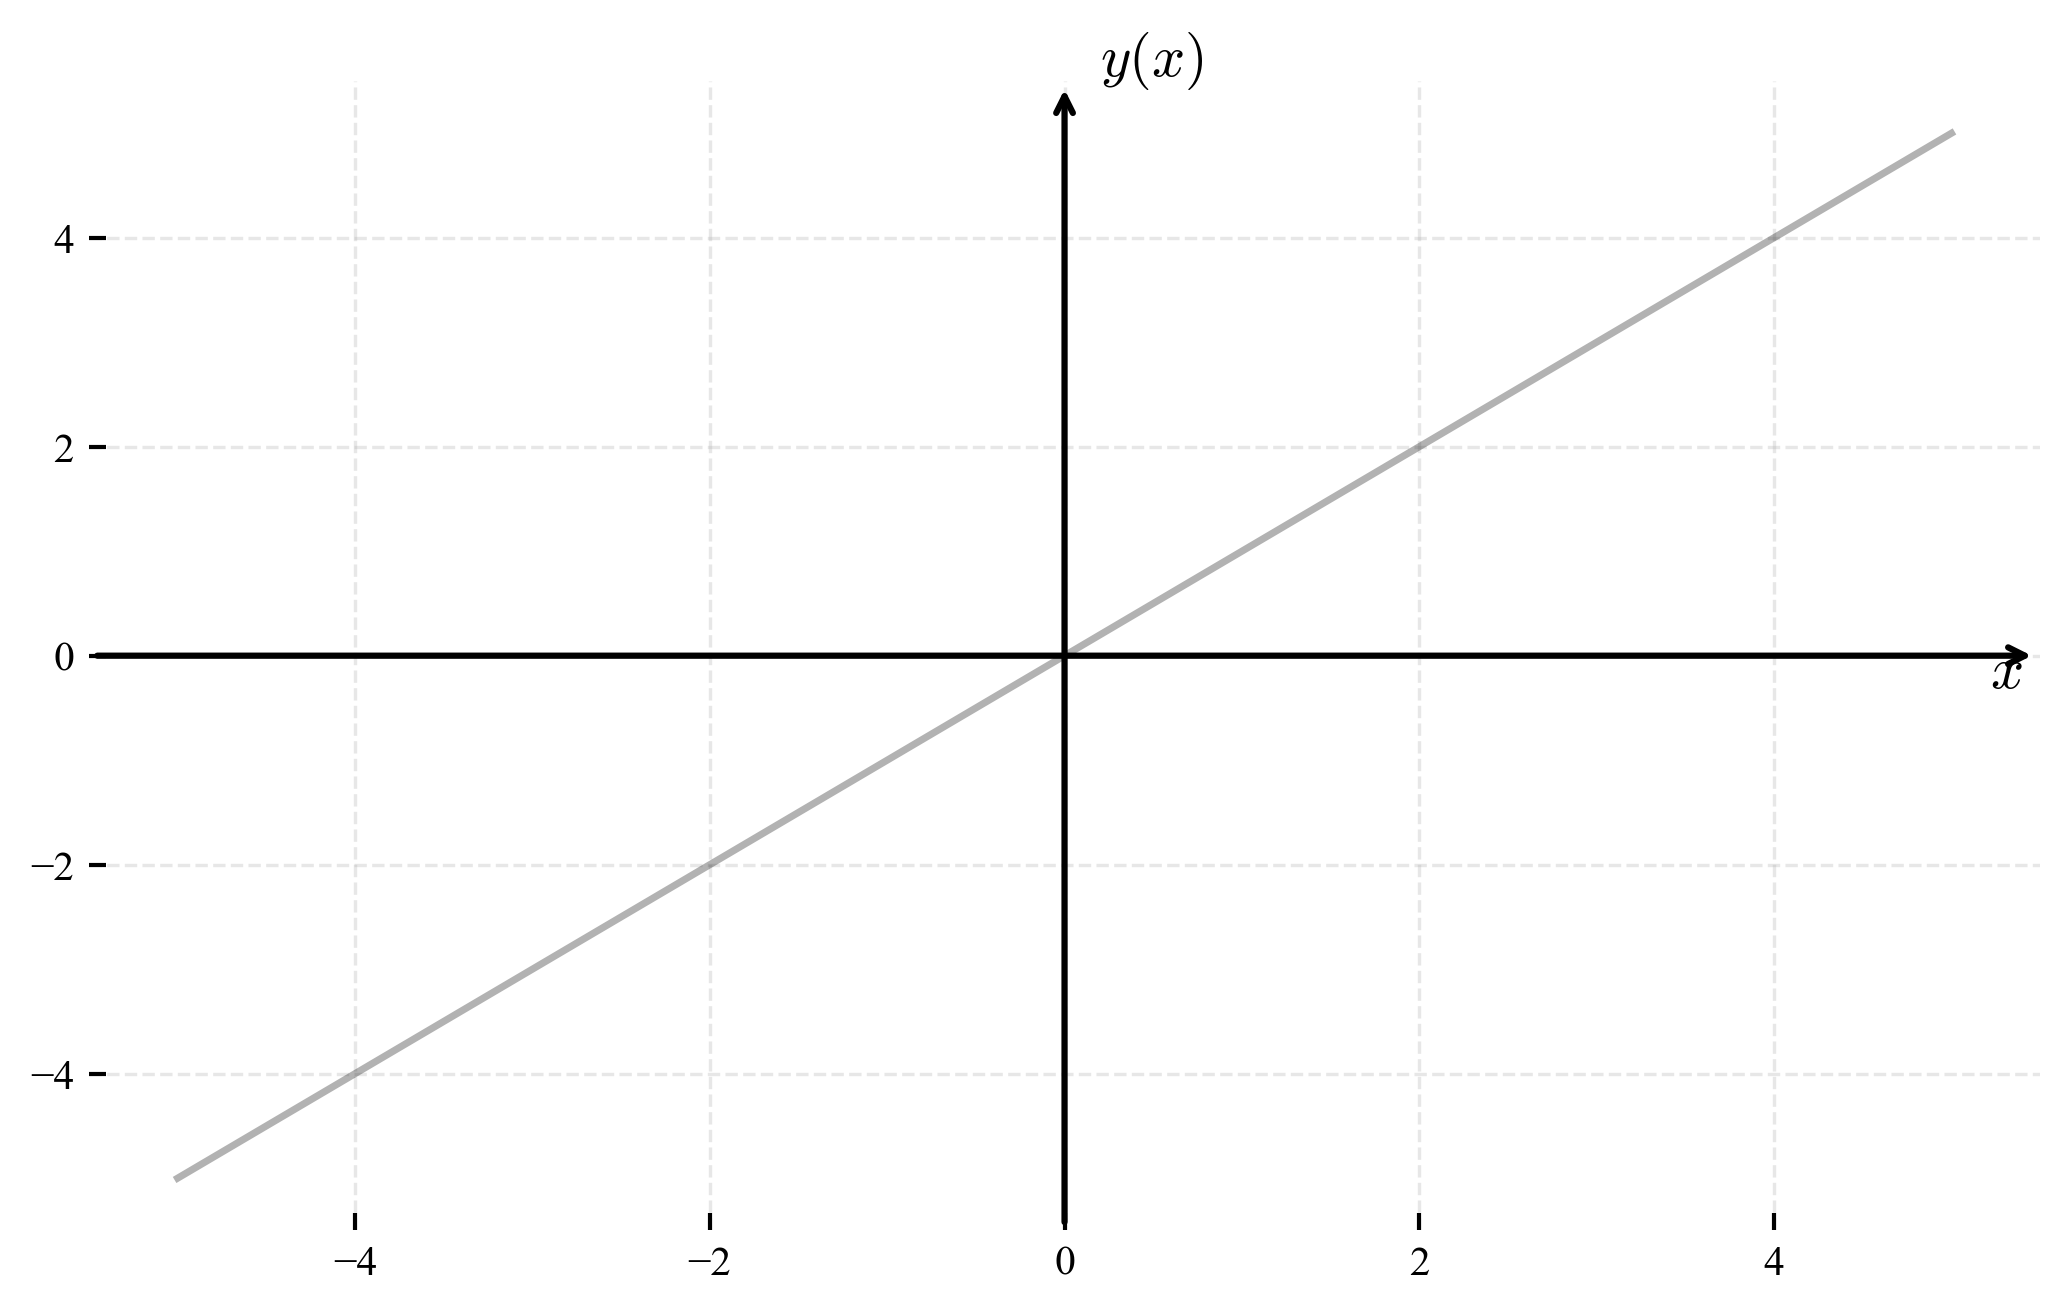
\includegraphics[width=0.7\textwidth]{5_figures/chapter5/linear.png}
        \caption{Representation of a linear function $y(x) = a \; x + b$. Examples of these are the force and displacement in a wire as given by Hooke's law $F(x) = k \; x$.}
        \label{fig:linear1}
    \end{subfigure}

    \vspace{1.2em}

    % ----------- Subfigure 2 -----------
    \begin{subfigure}{0.8\textwidth}
        \centering
        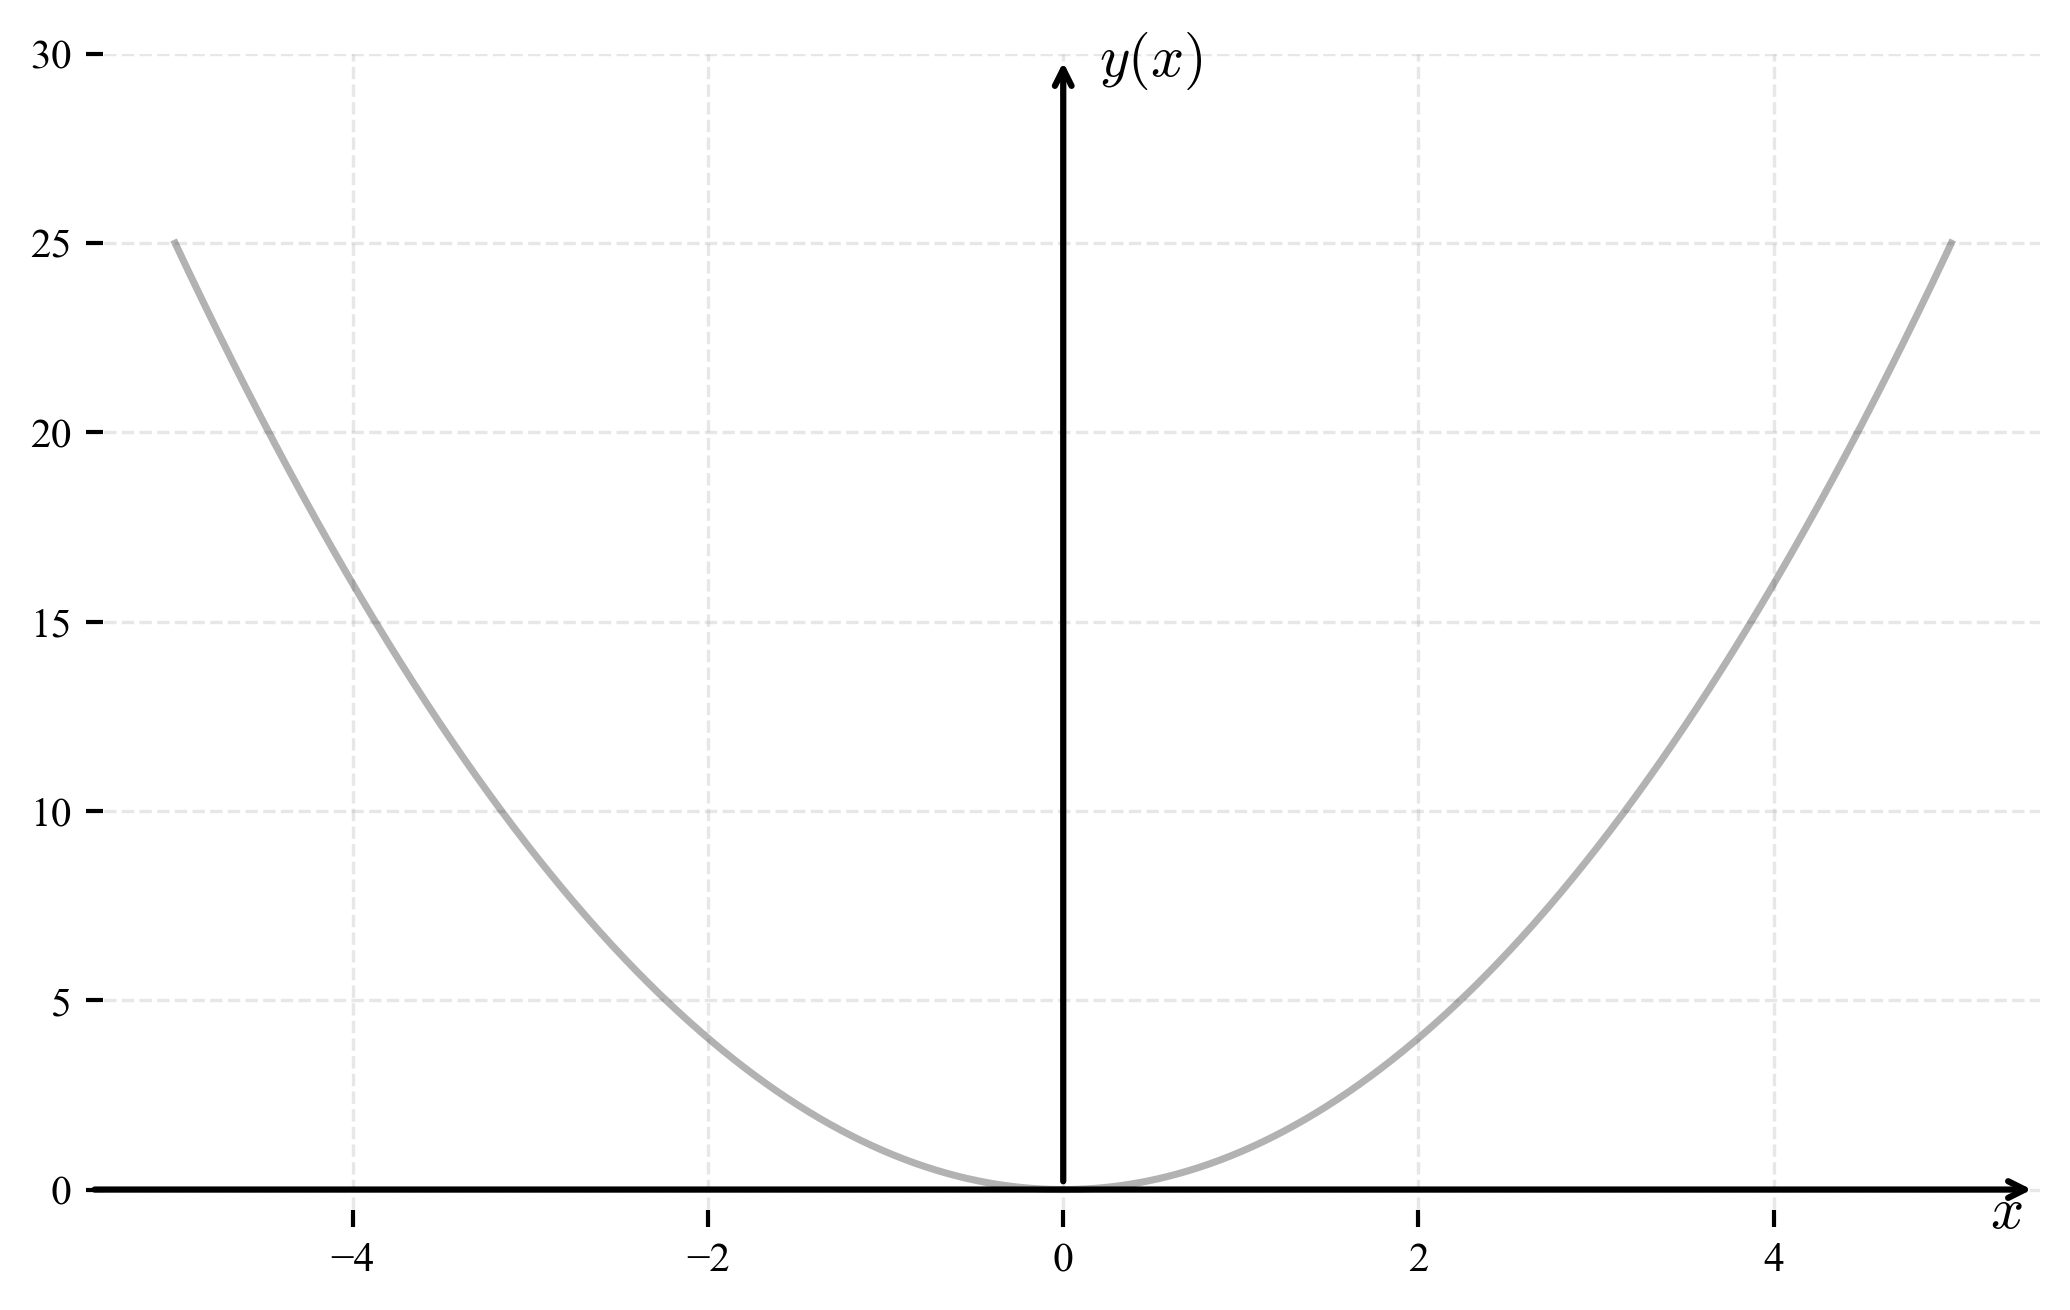
\includegraphics[width=0.7\textwidth]{5_figures/chapter5/quadratic.png}
        \caption{Representation of a quadratic function $y(x) = a \; x^2 + b \; x + c$. Example of these are, for instance, the displacement of a particle under constant acceleration in terms of time $x(t) = x_0 + v_0t + \tfrac{1}{2}at^2$.}
        \label{fig:quadratic1}
    \end{subfigure}

    \vspace{1.2em}

    % ----------- Subfigure 3 -----------
    \begin{subfigure}{0.8\textwidth}
        \centering
        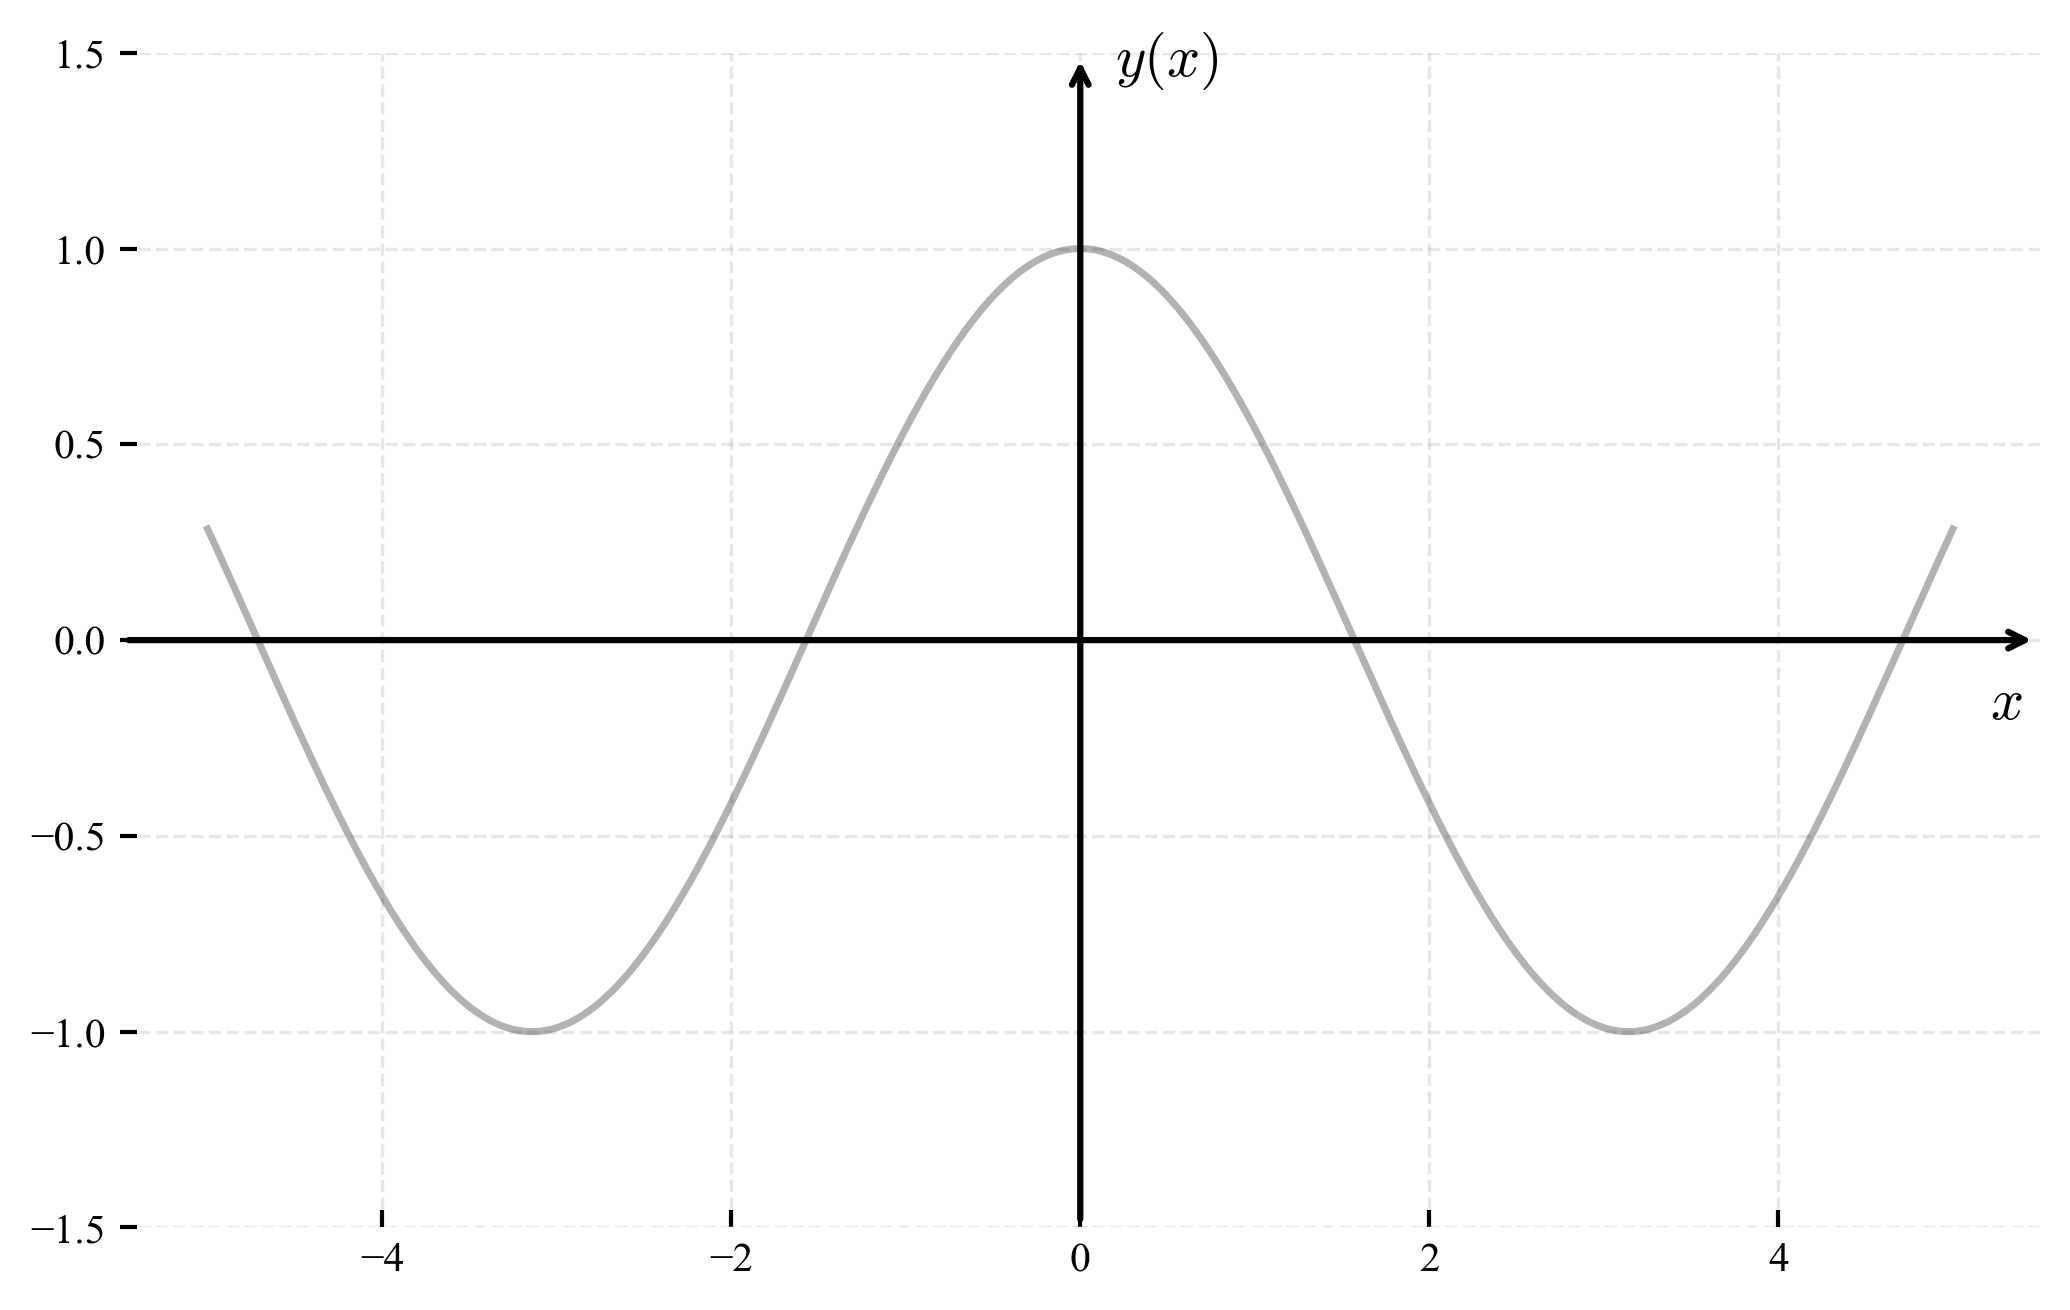
\includegraphics[width=0.7\textwidth]{5_figures/chapter5/sinusoidal.png}
        \caption{Representation of a sinusoidal function $y(x) = a \; \sin(x) + b \; \cos(x)$. Example of there are, for instance, the positon of a wirte with respect to time in a harmonic movement $x(t) = A\cos(\omega t + \phi).$}
        \label{fig:sinusoidal1}
    \end{subfigure}

    % ----------- Global caption -----------
    \caption{Representation of different dependencies between variables, commonly found in physical systems and daily life examples. As examples; linear, quadratic, and the sinusoidal.}
    \label{fig:functions1}

\end{figure}

% Statistical modelling ...............................................................................................
\section{Statistical modelling}

Classical mathematical models describe relationships between variables as \textit{exact} functional dependencies. In such \textit{deterministic} settings, once the input is specified, the output is uniquely determined. This perspective underlies much of classical physics and analysis, where laws are expressed in the form \(y = f(x)\). We normally refer to $x$ as the \textit{independent} variable, also sometimes as \textit{explanatory}, while $y$ is called the \textit{dependent}, or \textit{response} variable.

\medskip

However, real data rarely follows such idealized relationships. Measurements are subject to error, systems are influenced by unobserved factors, and natural phenomena exhibit intrinsic variability. As a result, identical inputs may lead to different observed outcomes. This motivates the introduction of randomness into models.

\medskip

The incorporation of uncertainty into scientific reasoning developed progressively, notably in the work of Laplace \cite{laplace_1812_theorie}, who interpreted probability as a measure of uncertainty, and later in the axiomatic formulation of Kolmogorov \cite{kolmogorov_1933_grundbegriffe}, which provided a rigorous mathematical foundation. Within this framework, observable quantities are modeled as random variables $X$, $Y$ and a statistical model takes the form
\begin{equation}
    Y = f(X) + \varepsilon \; ,
\end{equation}
where \(f(X)\) represents the systematic, deterministic component and \(\varepsilon\) is a random error term capturing deviations from the idealized relationship. This is why statistical models are referred to as \textit{stochastic}, to distinguish them from the purely deterministic mathematical models.

\medskip

The use of uppercase letters \(X, Y\), quite common in statistics textbooks, reflects this probabilistic viewpoint: they denote random variables, that is, quantities whose values are not fixed but distributed according to some underlying probability law. Observed data correspond to particular realizations—observations—of these variables, typically denoted by lowercase \(x_i, y_i\). This distinction, while not always emphasized in purely mathematical treatments, is central in statistics.

\begin{figure}[ht]

    \centering

    % ----------- Subfigure 1 -----------
    \begin{subfigure}{0.8\textwidth}
        \centering
        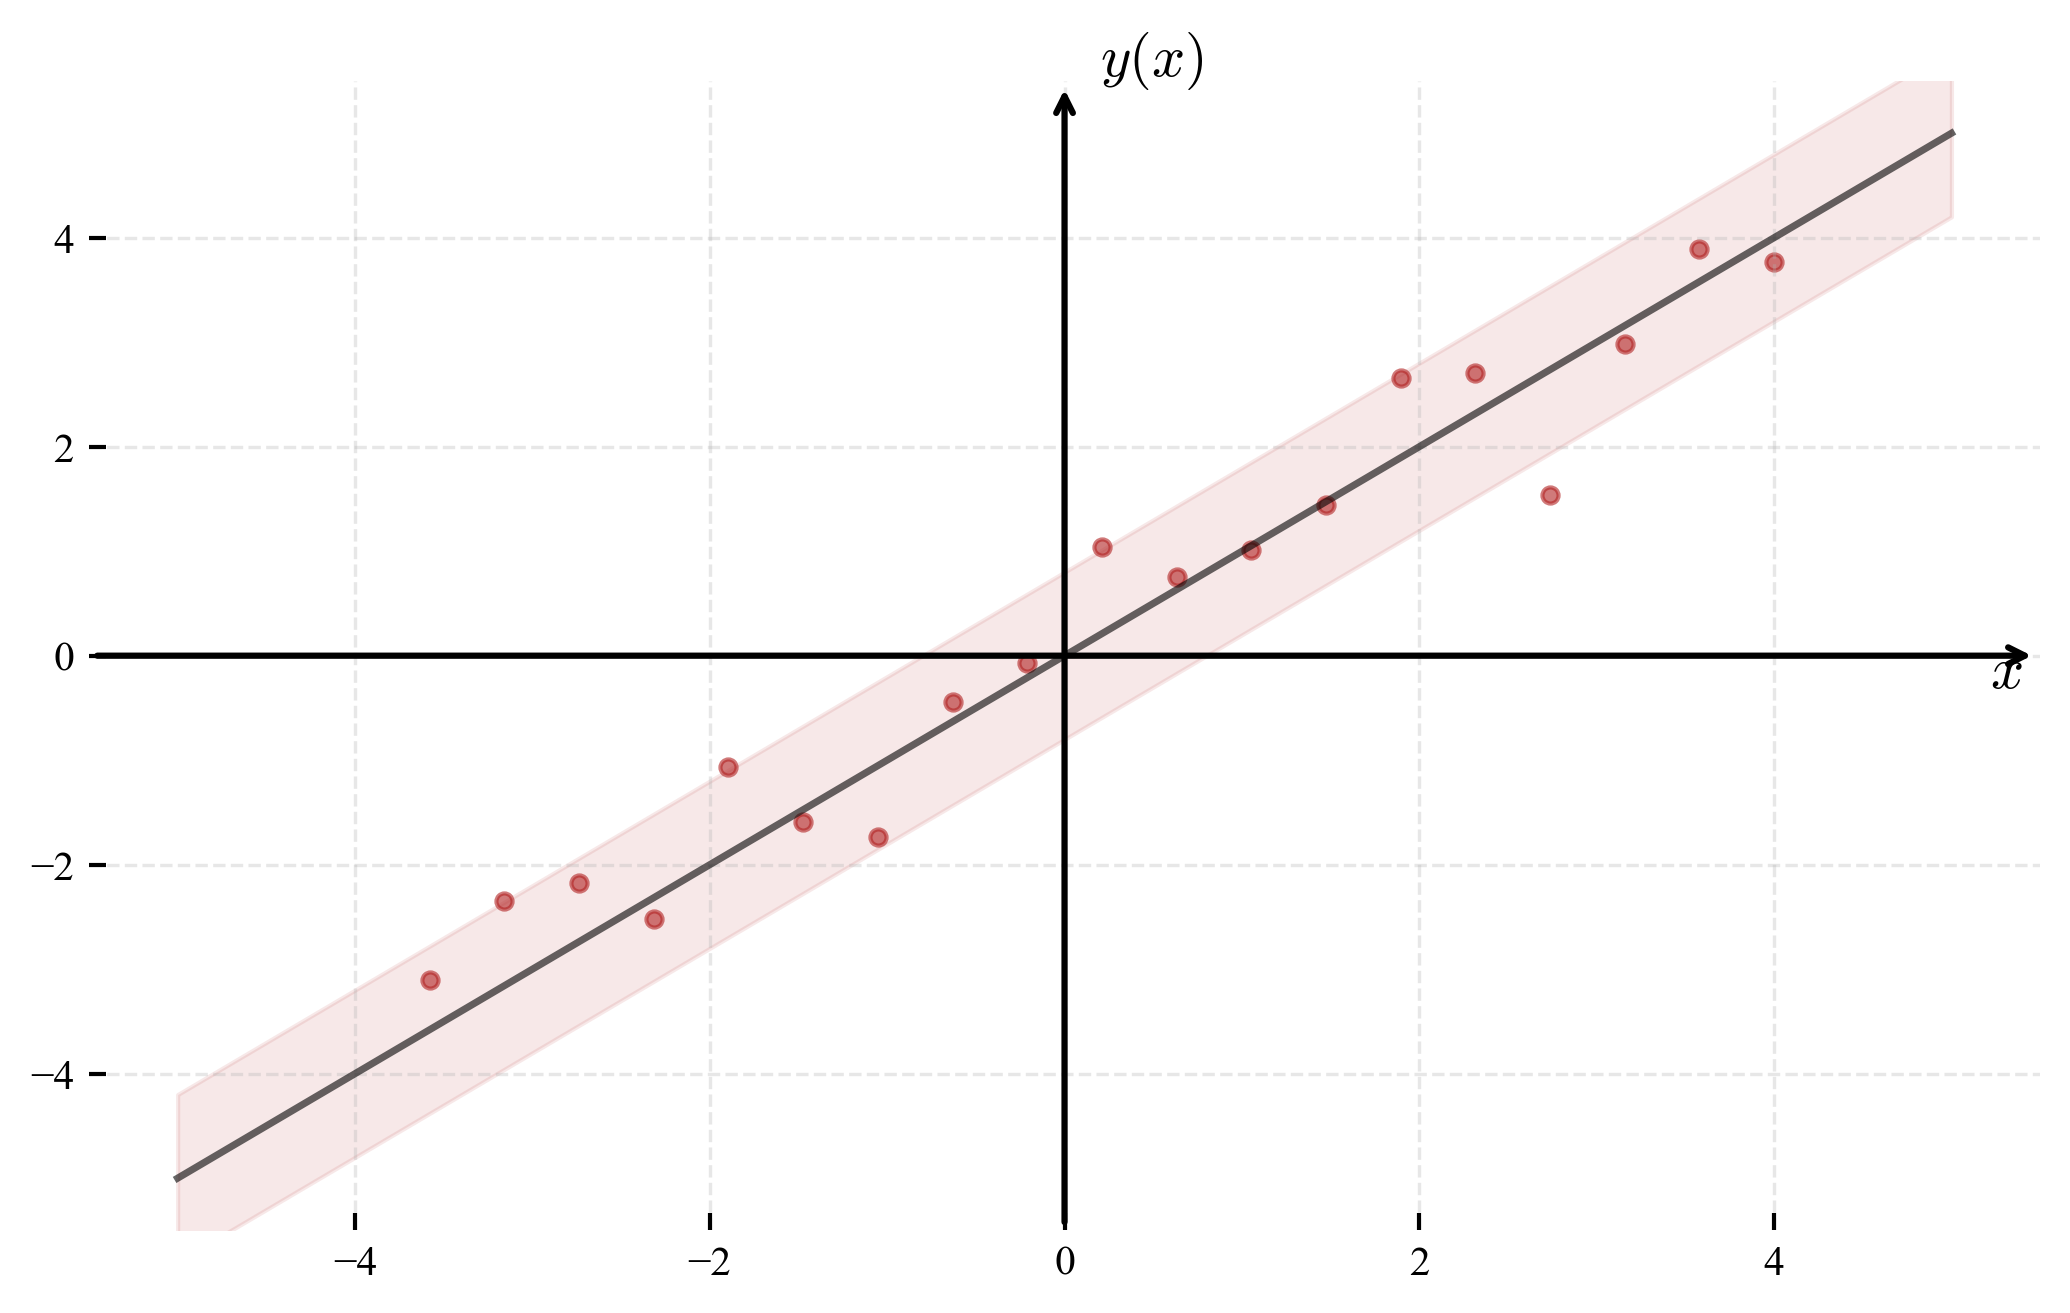
\includegraphics[width=0.7\textwidth]{5_figures/chapter5/linear_noise.png}
        \caption{Representation of a linear function with some statistical noise $y(x) = a \; x + b \pm \varepsilon$. Examples of these are the force and displacement in a wire as given by Hooke's law $F(x) = k \; x$.}
        \label{fig:linear2}
    \end{subfigure}

    \vspace{1.2em}

    % ----------- Subfigure 2 -----------
    \begin{subfigure}{0.8\textwidth}
        \centering
        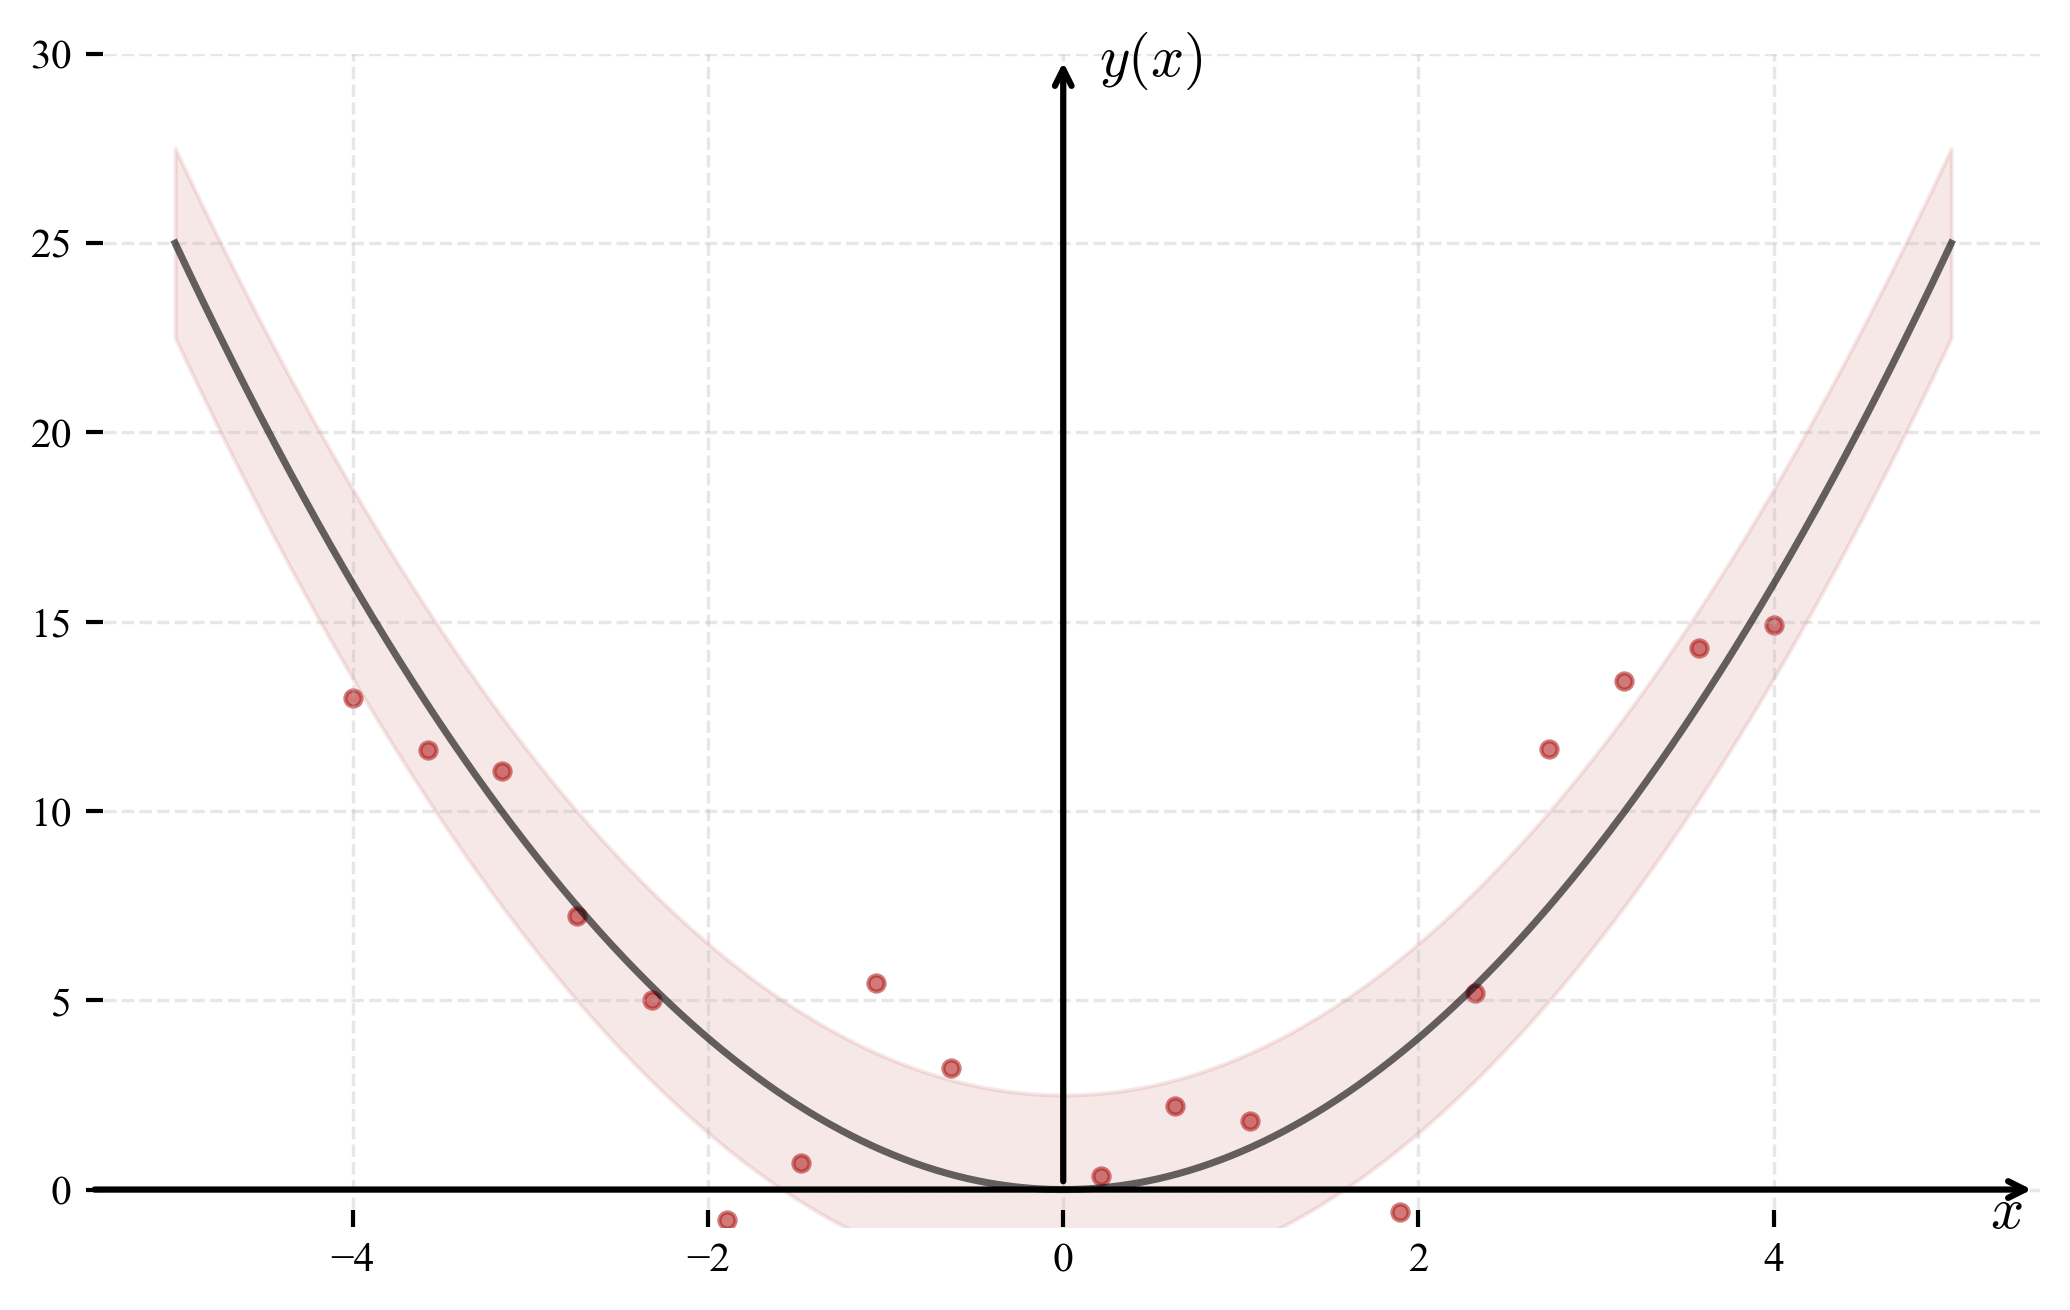
\includegraphics[width=0.7\textwidth]{5_figures/chapter5/quadratic_noise.png}
        \caption{Representation of a quadratic function $y(x) = a \; x^2 + b \; x + c \pm \varepsilon$. Example of these are, for instance, the displacement of a particle under constant acceleration in terms of time $x(t) = x_0 + v_0t + \tfrac{1}{2}at^2$.}
        \label{fig:quadratic2}
    \end{subfigure}

    \vspace{1.2em}

    % ----------- Subfigure 3 -----------
    \begin{subfigure}{0.8\textwidth}
        \centering
        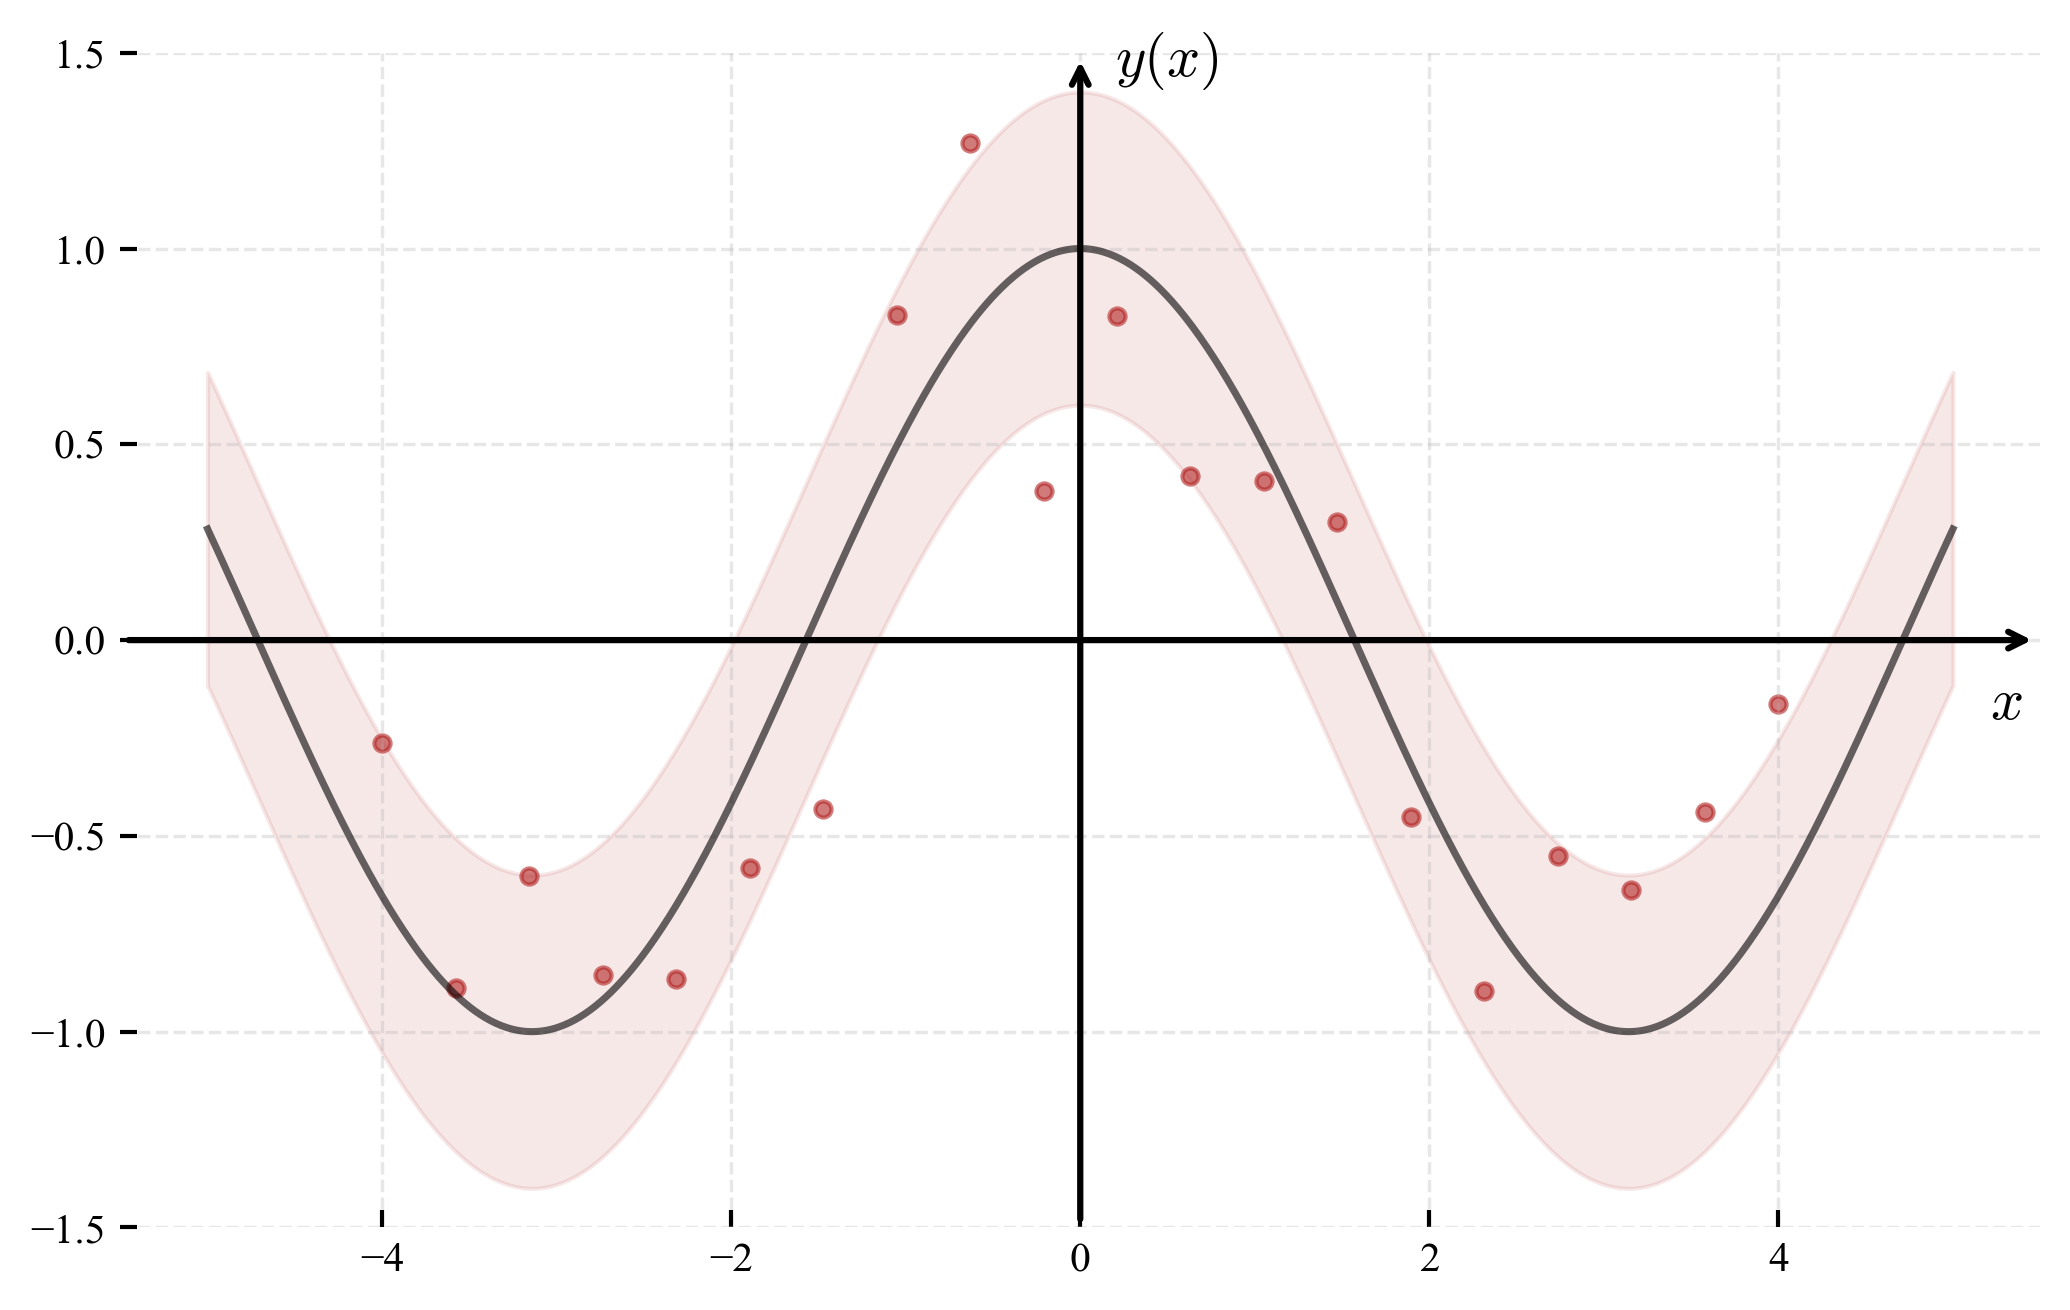
\includegraphics[width=0.7\textwidth]{5_figures/chapter5/sinusoidal_noise.png}
        \caption{Representation of a sinusoidal function $y(x) = a \; \sin(x) + b \; \cos(x) \pm \varepsilon$. Example of there are, for instance, the positon of a wirte with respect to time in a harmonic movement $x(t) = A\cos(\omega t + \phi).$}
        \label{fig:sinusoidal2}
    \end{subfigure}

    % ----------- Global caption -----------
    \caption{Representation of different dependencies between variables, with some statistical noise to differentiate from deterministic, exact mathematical models. The red dots represent observations following that correlation plus the statistical fluctuations.}
    \label{fig:functions2}

\end{figure}

% Linear Regression ...................................................................................................
\section{Linear Regression}

The concept of regression originates in the work of Galton \cite{galton_1886_regression}, who observed that extreme characteristics in parents tend to be less extreme in their offspring, a phenomenon he termed ``regression toward mediocrity.'' This empirical insight was later formalized and extended through the development of correlation and regression analysis by Pearson \cite{pearson_1895_contributions}, and placed within a broader probabilistic framework by Fisher \cite{fisher_1925_statistical}.

\medskip

A natural starting point, and among the simplest behaviors, is the \textit{linear}. This leads to the simple linear regression model. In purely mathematical contexts, linear relation is written in the form
\begin{equation}
    y(x) = ax + b + \varepsilon \; ,
\end{equation}

where lowercase notation emphasizes deterministic functions evaluated at specific inputs. The statistical formulation, instead, distinguishes between random variables \(X, Y\) and their realizations, and often uses the notation \(\beta_0, \beta_1\) to denote unknown parameters to be estimated. Both representations describe the same underlying idea, but reflect different conceptual perspectives: deterministic versus probabilistic.
\begin{equation}
    Y = \beta_0 + \beta_1 X + \varepsilon \; .
\end{equation}

In this formulation, \(\beta_0\) represents a baseline level or \textit{intercept}, while \(\beta_1\) quantifies the average change in \(Y\) associated with a unit change in \(X\), also known as \textit{slope}. The error term \(\varepsilon\) captures all sources of variation not explained by the linear relationship.

\medskip

Having specified a model, one must determine how well it describes the observed data. In practice, the values predicted by a model rarely coincide exactly with observations. The differences between observed values $y_i$ and the ones predicted by the model $\hat{y}_i$ are called \textit{residuals}:
\begin{equation}
    e_i = y_i - \hat{y}_i \; .
\end{equation}

These residuals provide a quantitative measure of the discrepancy between the model and reality. The problem of estimation may then be formulated as one of finding parameters that make these discrepancies—the residuals—as small as possible.

\medskip

For that purpose, a mathematical quantity commonly defined is the \textit{sum of squared residuals}:
\[
\mathrm{RSS} = \sum_{i=1}^n (y_i - \hat{y}_i)^2.
\]

A model which is very accurate will produce predictions very close to the observations, hence producing a very small sum of residuals. This principle, known as the method of least squares, was first introduced by Legendre \cite{legendre_1805_least} in the context of astronomical calculations, and later given a probabilistic justification by Gauss \cite{gauss_1809_theoria}, who showed that it arises naturally when observational errors are normally distributed. Through his work \textit{"Theoria motus corporum coelestium"}, trying to describe planetary motions, he developed this method of least squares, building a meeting point between geometry, algebra, and probability.

\medskip

The validity and interpretation of the resulting estimates rely on several assumptions:

\begin{itemize}

\item \textbf{Linearity:} the conditional mean is a linear function of \(X\):
    \[
        \mathbb{E}[Y \mid X=x] = \beta_0 + \beta_1 x.
    \]
    This means that, on average, \(Y\) changes at a constant rate as \(X\) changes. The data may be scattered, but the underlying trend follows a straight line.

\item \textbf{Independence:} the error terms are independent:
    \[
        \varepsilon_i \;\text{independent of}\; \varepsilon_j \quad (i \neq j).
    \]
    This means that the error made for one observation does not influence the error for another. In simple terms, knowing one data point does not give information about the error in another.

\item \textbf{Homoscedasticity:} the variance of the errors is constant:
    \[
        \mathrm{Var}(\varepsilon_i \mid X) = \sigma^2.
    \]
    This means that the spread of the data around the regression line is roughly the same for all values of \(X\). The variability does not increase or decrease as \(X\) changes.

\item \textbf{Normality:} the errors follow a normal distribution:
    \[
        \varepsilon_i \sim \mathcal{N}(0,\sigma^2).
    \]
    This means that most errors are small, large deviations are rare, and positive and negative errors are equally likely. This assumption is mainly important when making statistical inference (e.g. confidence intervals, tests).

\end{itemize}

These assumptions do not merely simplify analysis; they determine the conditions under which the model provides reliable inference.

% Covariance and Correlation ..........................................................................................
\section{Covariance and Correlation}

Beyond modelling the relationship between a response and a predictor, it is often of interest to quantify the degree to which two variables vary together. The earliest systematic attempts to measure such dependence arose in the late nineteenth century, notably in the work of Pearson \cite{pearson_1895_contributions}, who developed the concepts of covariance and correlation as tools for studying biological and social data.

\medskip

\textbf{Covariance:}

\medskip

Covariance provides a measure of joint variability between two random variables \(X, Y\):
\begin{equation}
    \mathrm{Cov}(X,Y) = \mathbb{E}[(X-\mathbb{E}X)(Y-\mathbb{E}Y)] \; .
\end{equation}

A \textit{positive} covariance indicates that the variables tend to \textit{increase together}, while a \textit{negative} value indicates \textit{opposite tendencies}. However, covariance depends on the scale of measurement and is therefore difficult to interpret in isolation.

To illustrate the computation of covariance, consider two short data sets:
\[
    x = (1,2,3), \quad y = (2,4,6).
\]
Their sample means are \(\bar{x} = 2\) and \(\bar{y} = 4\). The covariance is obtained by averaging the products of deviations from the means:
\[
    \mathrm{Cov}(X,Y) = \frac{1}{n} \sum_{i=1}^n (x_i - \bar{x})(y_i - \bar{y}).
\]
Substituting the values:
\[
    \mathrm{Cov}(X,Y) = \frac{1}{3}\big[(-1)(-2) + (0)(0) + (1)(2)\big] = \frac{4}{3}.
\]
This positive value reflects the fact that the variables increase together. In general, larger covariance indicates stronger joint variation, while values near zero suggest weak or no linear relationship.

\medskip

\textbf{Correlation:}

\medskip

To address the scale dependence, we can define the correlation coefficient, which normalizes covariance with the variances of both variables:
\begin{equation}
    \rho = \frac{\mathrm{Cov}(X,Y)}{\sigma_X \sigma_Y} \; .
\end{equation}

\medskip

As we discusseed in Chapter \ref{chapter1} and Chapter \ref{chapter3} population quantities such as \(\rho\) are typically unknown, and must be estimated from data. The most common estimator for the correlation is Pearson’s \textit{sample correlation coefficient}:
\begin{equation}
    r = \frac{\sum (x_i-\bar{x})(y_i-\bar{y})}{\sqrt{\sum (x_i-\bar{x})^2}\sqrt{\sum (y_i-\bar{y})^2}} \; .
\end{equation}

While Pearson’s coefficient measures linear association, alternative measures have been proposed to capture more general forms of dependence. In particular, Spearman \cite{spearman_1904_association} introduced a rank-based correlation that is sensitive to monotonic relationships and less affected by outliers.

\medskip

A striking illustration of the limitations of summary statistics is provided by Anscombe \cite{anscombe_1973_graphs}, who exhibited datasets with identical means, variances, correlations, and regression lines, yet radically different graphical structures. This example underscores the importance of complementing numerical measures with visualization.

\begin{figure}[ht]
    \centering
    
\includegraphics[width=0.8\textwidth]{5_figures/chapter5/anscombe.png}
    \caption{Representation of Anscombe's quartet (from English statistician Francis John Anscombe, 1918 – 2001), illustrating the limitations of summary statistics. All four datasets have exact same statistics and correlation values, while having clear different dependencies.}
    \label{fig:anscombe}
\end{figure}

% Multiple linear regression ..........................................................................................
\section{Multiple linear regression}

In many applications, a response variable depends on several factors simultaneously. Extending the linear model to incorporate multiple predictors leads to the multiple linear regression model:
\[
Y = \beta_0 + \beta_1 X_1 + \cdots + \beta_p X_p + \varepsilon.
\]

This generalization reflects the complexity of real-world phenomena, where outcomes are rarely determined by a single variable. Each coefficient \(\beta_j\) represents the effect of the corresponding predictor \(X_j\), holding all other variables fixed. In this sense, the model allows us to isolate the contribution of each variable while accounting for the presence of others.

\medskip

Historically, such models emerged as data collection expanded in scope and complexity during the late nineteenth and early twentieth centuries, particularly in biology, economics, and the social sciences. The work of Fisher \cite{fisher_1925_statistical} was instrumental in formalizing methods for analyzing systems influenced by multiple factors, especially in the context of experimental design.

\medskip

From a mathematical perspective, this model can be viewed as a natural extension of functions of a single variable to functions of several variables, as studied in multivariable calculus. In that setting, one considers functions of the form \(y = f(x_1, x_2, \dots, x_p)\), where the output depends jointly on several inputs. The linear regression model corresponds to the simplest such case, where the function is linear in each variable.

\medskip

Concrete examples arise in many domains. In economics, one may model income as a function of education, experience, and age. In physics, the pressure of a gas may depend on temperature and volume. In epidemiology, the risk of disease may be related to multiple environmental and genetic factors. In each case, the goal is to understand how several variables jointly influence an outcome.

\medskip

In compact form, the model can be written using matrix notation:
\[
\mathbf{y} = \mathbf{X}\boldsymbol{\beta} + \boldsymbol{\varepsilon},
\]
which reveals its connection to linear algebra. In this setting, estimation by least squares corresponds to projecting the observed data onto the subspace spanned by the columns of \(\mathbf{X}\) \cite{strang_2016_linear}. This geometric interpretation provides additional insight into the structure of the problem, linking statistical estimation with concepts from vector spaces and orthogonality.
